\documentclass[tikz,border=10pt]{standalone}
\usepackage{tikz}
\usetikzlibrary{arrows.meta,positioning}

\tikzset{
  sfgsource/.style={circle, draw=green!60!black, line width=1.2pt, minimum size=0.9cm, inner sep=0pt},
  sfgnode/.style={circle, draw=purple!70!black, line width=1.2pt, minimum size=0.9cm, inner sep=0pt},
  sfgsink/.style={circle, draw=red!70!black, line width=1.2pt, minimum size=0.9cm, inner sep=0pt},
  sfgedge/.style={->, line width=1.2pt, draw=black!80, >=Stealth},
  gain/.style={font=\small\itshape, fill=white, inner sep=1pt}
}

\begin{document}
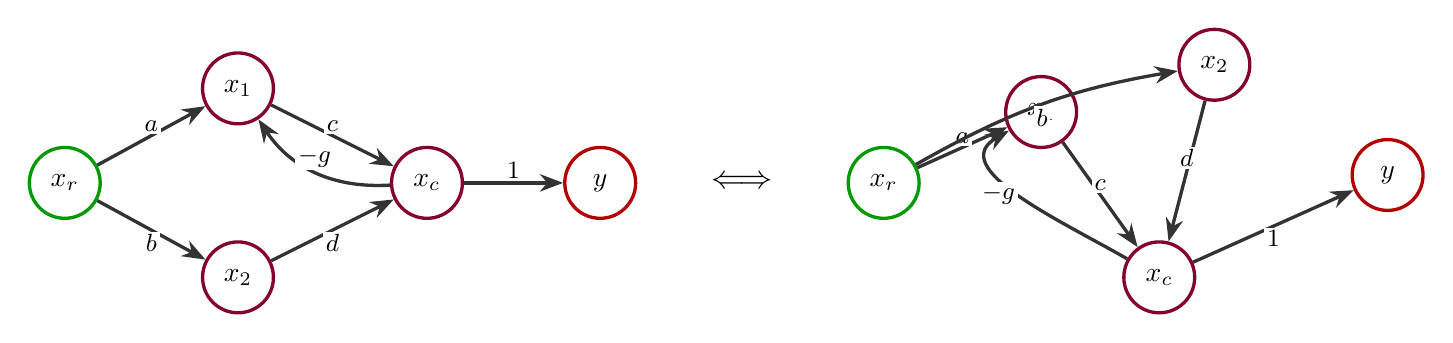
\begin{tikzpicture}
  % left
  \node[sfgsource] (r1) at (0,0) {$x_r$};
  \node[sfgnode] (x1) at (2.2,1.2) {$x_1$};
  \node[sfgnode] (x2) at (2.2,-1.2) {$x_2$};
  \node[sfgnode] (xc1) at (4.6,0) {$x_c$};
  \node[sfgsink] (y1) at (6.8,0) {$y$};
  \draw[sfgedge] (r1) -- node[gain, above] {$a$} (x1);
  \draw[sfgedge] (r1) -- node[gain, below] {$b$} (x2);
  \draw[sfgedge] (x1) -- node[gain, above] {$c$} (xc1);
  \draw[sfgedge] (x2) -- node[gain, below] {$d$} (xc1);
  \draw[sfgedge] (xc1) -- node[gain, above] {$1$} (y1);
  \draw[sfgedge, bend left=30] (xc1) to node[gain, above] {$-g$} (x1);

  \node[font=\large] at (8.6,0) {$\Longleftrightarrow$};

  % right
  \node[sfgsource] (r2) at (10.4,0) {$x_r$};
  \node[sfgnode] (x1b) at (12.4,0.9) {$x_1$};
  \node[sfgnode] (x2b) at (14.6,1.5) {$x_2$};
  \node[sfgnode] (xcb) at (13.9,-1.2) {$x_c$};
  \node[sfgsink] (y2) at (16.8,0.1) {$y$};
  \draw[sfgedge] (r2) -- node[gain, above] {$a$} (x1b);
  \draw[sfgedge, bend left=10] (r2) to node[gain, below] {$b$} (x2b);
  \draw[sfgedge] (x1b) -- node[gain, above] {$c$} (xcb);
  \draw[sfgedge] (x2b) -- node[gain, above] {$d$} (xcb);
  \draw[sfgedge] (xcb) -- node[gain, below] {$1$} (y2);
  \draw[sfgedge, out=150, in=210, looseness=1.1] (xcb) to node[gain, left] {$-g$} (x1b);
\end{tikzpicture}
\end{document}
